%%%% Draft paper %%%%
% Title:
%  - Guidance for Autonomous Precision Landing on Airless Bodies
%
% Authors: 
%  - Ingo Gerth, Erwin Mooij
%
% Contact: 
%  - ingo@gerth-ac.de, e.mooij@tudelft.nl
%
% Git repository:
%  - https://github.com/tehingo/gnc-paper.git 
%
% Compiling:
%  - Make sure the files are encoded as UTF8
%  - Use lualatex, bibtex for bibliography, makeindex for nomenclature
%
% To execute AIAA old-school nomenclature run:
%  - makeindex -s nomencl.ist -o advanced_example.gls advanced_example.glo
%
% General note:
%  - Original AIAA template is *very* out-dated. Updated with recent packages
%  - .PDF upload is allowed
%
\documentclass[%
    % draft, % mostly for faster compilation
    % submit, % AIAA option, increases line space and font size
]{aiaa-tc}

%---------------------L E G A L    N O T I C E --------------------------------%
% Preamble.tex
% Copyright 2014 Ingo Gerth
%
% This is file `aiaa-pretty.cls'. It is based off of advanced_example.tex, which
% was written (c) 2004 by Bil Kleb, Bill Wood, and Erich Knauseberger.
%
% Editing this file is perfectly permitted by the distributing author, Ingo
% Gerth, but changing the name is recommended before making any major changes.
% 
% This work may be distributed and/or modified under the
% conditions of the LaTeX Project Public License, either version 1.3
% of this license or (at your option) any later version.
% The latest version of this license is in
%   http://www.latex-project.org/lppl.txt
% and version 1.3 or later is part of all distributions of LaTeX
% version 2005/12/01 or later.
%
% This work has the LPPL maintenance status 'maintained'.
% 
% The Current Maintainer of this work is Ingo Gerth
%
% This work is based on the official AIAA LaTeX template, version 3.6.1.
% The class aiaa-tc remains completely unchanged.
% The only changes are: 
%  * updated and simplified this template file for the body
%  * added the file Preamble.tex
%    - Removed obsolete packages
%    - Added new ones, replaced obsolete ones by more recent packages
%    - For details, please see the file Preamble.tex that tracks all changes
%  * Added a few hints here and there
%
% Description: LaTeX template for AIAA papers
% Keywords: LaTeX, template, AIAA
% Author (Preamble.tex): Ingo Gerth
% Author (advanced_example.tex): Bil Kleb, Bill Wood, Erich Knausenberger
% Maintainer: Ingo Gerth
% Version: 1.1 <21 January 2014>
%---------------------L E G A L    N O T I C E --------------------------------%



% ---------------------------------------------------------------------------- %
%%% Below: original AIAA packages, keeping for compatibility ----------------- %
%% (IG 2013-11-08: package below is obsolete, replace by cleveref)
% \usepackage{varioref}%  smart page, figure, table, and equation referencing
%
%% (IG 2013-11-08: This is bad practice, do not use)
% \usepackage{wrapfig}%   wrap figures/tables in text (i.e., Di Vinci style)
%
%% (IG 2013-11-08: Unnecessary, just place table in a minipage)
% \usepackage{threeparttable}% tables with footnotes
%
%% (IG 2013-11-08: obsolete package, use siunitx S column type)
% \usepackage{dcolumn}%   decimal-aligned tabular math columns
%  \newcolumntype{d}{D{.}{.}{-1}}
%
%% (IG 2013-11-08: obsolete package, consider using glossaries instead)
\usepackage{nomencl}%   nomenclature generation via makeindex
 \makeindex
 \makenomenclature
%
%% (IG 2013-11-08: obsolete package, use successor subfig)
% \usepackage{subfigure}% subcaptions for subfigures
% \usepackage{subfigmat}% matrices of similar subfigures, aka small mulitples
%
%% (IG 2013-11-08: package obsolete, use lettrine)
% \usepackage[dvips]{dropping}% alternative dropped capital package
%
%% (IG 2013-11-08: below is unchanged, packages are good)
\usepackage[colorlinks]{hyperref}%  hyperlinks [must be loaded after dropping]
\usepackage[american]{babel}
\usepackage{fancyvrb}%  extended verbatim environments
 \fvset{fontsize=\footnotesize,xleftmargin=2em}
\usepackage{lettrine}%  dropped capital letter at beginning of paragraph
% ----------------- above: original AIAA packages, keeping for compatibility %%%
% ---------------------------------------------------------------------------- %


% ---------------------------------------------------------------------------- %
%%% Below: Package additions / replacements with newer packages -------------- %
% \usepackage{fontspec} % needed for running the lualatex compiler
\usepackage{xspace} % to get the spacing after macros right  
\usepackage{mparhack} % get marginpar right
\usepackage{fixltx2e} % fixes some LaTeX stuff 
\usepackage{microtype} % Microtypographic enhancements
% \usepackage[english]{selnolig} % Suppress bad ligatures
\usepackage{siunitx} % Proper unity typesetting
    \sisetup{exponent-product=\cdot, per-mode=symbol} % get / instead of ^{-1}
\usepackage{amsmath,amsfonts,amssymb} % Primary math packages
\usepackage{mathtools} % Important math fixes and extensions
% \usepackage{lualatex-math} % Math fixes for LuaLaTeX compiler
\usepackage{etoolbox} % Needed to write new commands properly
\usepackage{xargs} % idem
\usepackage{xparse} % idem
\usepackage[bottom]{footmisc} % Avoid that figures show up *below* footnotes
\usepackage{subfig} % Replacement for subfigure
\usepackage{booktabs} % Publication-quality tables
\usepackage{pgfplots} % Publication-quality plots
    \pgfplotsset{compat=1.9}
\usepackage{tikz} % Program vector drawings
    \usetikzlibrary{calc,decorations.pathreplacing,shapes,arrows,positioning,shadows,patterns}
    \pgfdeclarelayer{bg}    % declare background layer
    \pgfsetlayers{bg,main}  % set the order of the layers (main is the standard layer)
% -------------- Above: Package additions / replacements with newer packages %%%
% ---------------------------------------------------------------------------- %

% Automatically import hyphenation exceptions:
% - uncomment and adapt to your file path
% - fixes some hyphenations that babel usually gets wrong
% \input{/usr/local/texlive/2013/texmf-dist/tex/generic/hyphenex/ushyphex.tex}

% Mark bad boxes despite final option
% \overfullrule=1mm

% Abbreviations
\newcommand\eg{\emph{e.g.}\xspace}
\newcommand\ie{\emph{i.e.}\xspace}
\newcommand\wrt{wrt.\xspace}
\newcommand\com{c.o.m.\xspace}

% New math commands
\newcommand\const{\text{const.\xspace}}
\newcommand\minimize{\text{minimize}}
\providecommand{\abs}[1]{\lvert#1\rvert}
\providecommand{\norm}[1]{\lVert#1\rVert}
\newcommand{\transpose}[1]{\ensuremath{{#1}^{\intercal}}}
\newcommand{\ed}{\ensuremath{\operatorname{d}}}
\newcommand{\trans}[1]{\ensuremath{{#1}^{\mathlarger\intercal}}}


%%% Further packages, use only when need ----------------------------------- %%% 
% \usepackage{minted} % Code listings with syntax highlighting



\title{Guidance for Autonomous Precision Landing on Atmosphereless Bodies}

\author{
 Ingo Gerth\thanks{%
     Graduate student, Section of Astrodynamics and
     Space Missions. AIAA student member.%
     % Intern at ESA ESTEC, D/HSO-IL (Lunar Lander Office). 
     %
 }
 \ and Erwin Mooij\thanks{Assistant professor, Section of Astrodynamics and Space Missions.  Associate
     Fellow, AIAA.}\\
 {\normalsize\itshape
  Delft University of Technology, Delft, The Netherlands, 2629\,HS}
}

\AIAAsubmitinfo{Landing Guidance Methods, Gerth and Mooij}

% Data used by 'handcarry' option
\AIAApapernumber{YEAR-NUMBER}
\AIAAconference{Conference Name, Date, and Location}
\AIAAcopyright{\AIAAcopyrightD{YEAR}}

% Define commands to assure consistent treatment throughout document
\newcommand{\eqnref}[1]{(\ref{#1})}
\newcommand{\class}[1]{\texttt{#1}}
\newcommand{\package}[1]{\texttt{#1}}
\newcommand{\file}[1]{\texttt{#1}}
\newcommand{\BibTeX}{\textsc{Bib}\TeX}

\begin{document}

% Notations (see author_guide.pdf)
% --------------------------------
% Use "figure", "table" (small, written out)
% Table caption on top, figure below
% For citations, use Ref.~1 (inconsistent with above, but oh well...)
% For equations, use Eq.~1 (again, inconsistent...... well well well.)
% At beginning of sentence write out, e.g., Equation~1, Reference~1
% Express ranges with "to", eg. Eqs.~1 to~3.
% Put "periods and commas in quotation marks," but "exclamations not"!
% Use listings as this, that, and that (serial comma)
% If number of authors >= 6, say et al. in bibliography
% Label for sub floats: a), b), etc.
% For figure axes, use words

% Remarks on style (see author_guide.pdf)
% ---------------------------------------
% Use micrometer, not micron
% Graph within a graph is an inset, not insert
% Use alternatively, not alternately (unless something alternates)
% Whereas instead of while (unless referring to simultaneous events)
% Do not use essentially to mean approximately or effectively
% Do not use issue for euphemism of problem
% Data is plural, e.g., "data are" not "data is"
% Join prefixes such as non, sub, micro, multi, ultra with word, "submillimeter"
% Do not italicize i.e., e.g.
% Acknowledgment (without e after g, US style)

\maketitle

\begin{abstract}
    Two key technologies that will likely fly on next-generation planetary
    landers are hazard detection and avoidance (HDA) and vision-based
    navigation. The purpose of HDA is to make previously unsafe landing sites
    accessible by future vehicles, and to increase the safe landing probability
    overall. Vision-based navigation will enable to target specific landing
    sites more precisely and also plays an important role for HDA. This paper
    formulates requirements on the guidance system that derive from the needs of
    these new systems. After the introduction of a reference mission scenario
    with HDA and vision-based navigation in-the-loop, an extensive literature
    survey of the state-of-the-art in approach-phase guidance-algorithms is
    presented. This presents the methods under the angle of HDA-compatibility.
    The sheer number of papers mentioned here leads to the conclusion that
    trade-offs are challenging. It is recommended to do a down-selection from
    the papers presented here, and do a performance-based trade study for the
    particular test case under consideration with a few candidates. As an
    example, $E$-Guidance is presented for a Mercury- and a Moon-landing
    scenario. Because the results differ dramatically, it is concluded that it
    is essential to perform trade-offs on the actual mission scenario under
    study, and that trades cannot merely be based on references in the
    literature.  Because the proposed $E$-Guidance method is not satisfyingly
    robust, it is a goal of future research to improve upon this.
\end{abstract}

\printnomenclature

\section{Introduction}

\lettrine{H}{\textsc{istorically}} speaking, the success rate of robotic
planetary landers has been unsatisfyingly low. The cumulative probability of
failure based on historical data was about 20\,\% by the beginning of the last
decade.\cite{Strandmoe1999} This may in part be traced to the limited
capabilities of past systems: all landers were ``blind'', and were unable to
evade any surface hazards encountered. For much the same reason, the landing
precision of past vehicles was limited as well. For example, assuming an approach
without human intervention (which can be considered vision-based navigation), the
predicted landing ellipse for Apollo~12 measured \SI{13.3}{km} by
\SI{4.8}{km}.\cite{Bennett1970} 

To improve upon this, investigations for equipping future vehicles with landing
sensors to sense hazards and improve navigation solutions are carried out by
several agencies, especially as part of NASA's autonomous landing and hazard
avoidance technology (ALHAT) and ESA's Lunar Lander
projects.\cite{Epp2007,Rosa2011} These additions require to rethink the entire
landing guidance, navigation, and control (GNC) system. This paper focuses on
the impact on guidance. It presents a survey of suitable algorithms in the
literature.  Guidance is particularly affected by new constraints on the
trajectory, for example glide-slope constraints to keep the landing site in the
field of view (FOV) of a navigation camera or a hazard-detection lidar.

In recent years, renewed interest in lunar surface-exploration and the continued
investment into Mars-entry spacecraft has led to a great number of publications
in the field. It is a daunting task for designers to select the most suitable
guidance mode for their particular application from those available in the
literature.  In recent years, trades involving a selected few algorithms have
been presented by Sostaric and Rea (2005)\cite{Sostaric2005} and by Steinfeldt
et al.\ (2008).\cite{Steinfeldt2008} The last broad overview of the state-of-the
art in guidance modes was given by Pfeiffer (1968),\cite{Pfeiffer1968} which is
long outdated by today's standards. 

This paper presents a survey of most guidance algorithms for planetary landing
that have been published. It aims to define the needs for guidance if operated
in a hazard detection and avoidance (HDA) and precision-landing GNC-framework,
based on which a selection of promising algorithms is presented in detail. Less
applicable or immature modes are listed nevertheless to complete the picture.
$E$-Guidance is presented as a candidate for future missions. With its long
heritage, it serves as a good \emph{example} and benchmark.

First, the area of study is defined in Section~II, which entails the definition of
a reference scenario and the mathematical formulation of the guidance problem.
Next, Section~III introduces some trends in autonomous landing technology and
gives a brief analysis of their impact on the guidance system. The
state-of-the-art in approach-phase guidance-algorithms is then laid out in
Section~IV, which distinguishes between open-loop, explicit, and numerical
methods. To round off the discussion on guidance, the application of the
$E$-Guidance algorithm is demonstrated by an example in Section~V. The paper is
concluded by Section~VI, which also gives some recommendations and an outlook on
future work.


\section{Area of Study}

Guidance algorithms are usually tailored to a particular mission phase, and are
not generally applicable. To give a picture of a landing sequence and the phase
considered here, a reference based on the ESA Lunar Lander scenario is drawn
up.\cite{Fisackerly2012} This scenario is based on the heritage of previous
missions, most notably Apollo,\cite{Klumpp1974} and the terms introduced here
are thus common terminology and applicable to typical landings on atmosphereless
bodies of sufficient gravity.\cite{Paschall2009} Based on this, the guidance
problem can be formulated mathematically.


\subsection{Reference Scenario}

The reference scenario is shown in Figure~\ref{fig:scenario}. The mission is
assumed to start in a low lunar orbit (LLO). The descent begins with the descent
orbit insertion (DOI), which inserts the spacecraft into a Hohmann-transfer
orbit with a lowered periapsis above the landing site. In case of the ESA Lunar
Lander, the main braking phase is started at \SI{500}{km} downrange with the
powered descent initiation (PDI) maneuver. During this phase, most of the
orbital velocity is eliminated, bringing it down from about \SI{1630}{m/s} to
\SI{70}{m/s}. 

% \begin{figure}
%     \centering\small
%     \includegraphics[width=0.75\textwidth]{ReferenceScenario.png}
%     \caption{Reference mission scenario. Only approach phase algorithms are
%         considered. Adapted from Ref.~\citen{Delaune2010}}
%     \label{fig:scenario}
% \end{figure}

\begin{figure}
    \centering\small
    \begin{tikzpicture}[node distance={1.0cm and 1.0cm},>=latex]

        \draw (7.5, 0.5)node[rotate=0] {\includegraphics[width = 15cm]{surface2.png}};

        \draw[->] (0,0) -- (0,8);
        \draw[] (0,0) -- (15,0);

        \draw[->] (1,0) -- (1,8);
        \draw[->] (0,0.5) -- (15,0.5);
        \draw[->] (0,1) -- (15,1);

        \draw[dotted] (3,0) -- (3,8);
        \draw[dotted] (5,0) -- (5,8);
        \draw[dotted] (9,0) -- (9,8);
        \draw[dotted] (13,0) -- (13,8);
        \filldraw[fill = yellow](1,8.5)--(3,8.5) --(3,9)-- (1,9) --(1,9) -- (1,8.5);
        \filldraw[fill = orange](5,8.5)--(3,8.5) --(3,9)-- (5,9) --(5,8.5);
        \filldraw[fill = yellow](5,8.5)--(9,8.5) --(9,9)-- (5,9) --(5,8.5);
        \filldraw[fill = orange](9,8.5)--(13,8.5) --(13,9)-- (9,9) --(9,8.5);
        \filldraw[fill = yellow](13,8.5)--(15,8.5) --(15,9)-- (13,9) --(13,8.5);

        \filldraw[fill = lightgray](1,9)--(3,9) --(3,9.5)-- (1,9.5) -- (1,9);
        \filldraw[fill = gray](9,9)--(3,9) --(3,9.5)-- (9,9.5) --(9,9);
        \filldraw[fill = lightgray](9,9)--(15,9) --(15,9.5)-- (9,9.5) --(9,9);


        \draw (0,8)node[anchor=south] {\footnotesize $V$ };
        %\draw (0,5.8)node[anchor=south] {\footnotesize $[km/h]$ };
        \draw (1,8)node[anchor=south] {\footnotesize $h$};
        %\draw (1,5.8)node[anchor=south] {\footnotesize $[km]$ };
        \draw (15,0.5)node[anchor=south, draw, fill=white] {\footnotesize Time-to-go };
        \draw (15,1)node[anchor=south, fill=white] {\footnotesize Downrange };
        \draw (3,0.5)node[anchor=south, draw, fill=white] {\footnotesize 1 hour };
        \draw (3,1)node[anchor=south, fill=white] {\footnotesize 5500 km };
        \draw (5,0.5)node[anchor=south, draw, fill=white] {\footnotesize 12 min };
        \draw (5,1)node[anchor=south, fill=white] {\footnotesize 500 km };
        \draw (9,0.5)node[anchor=south, draw, fill=white] {\footnotesize 90 s };
        \draw (9,1)node[anchor=south, fill=white] {\footnotesize 2km};
        \draw (13,0.5)node[anchor=south , draw, fill=white] {\footnotesize 20 s };
        \draw (11.5,1)node[anchor=south] {\footnotesize Landing site };

        \draw (2,9.25)node[] {\footnotesize LLO };
        \draw (6,9.25)node[] {\footnotesize Descent };
        \draw (12,9.25)node[] {\footnotesize Landing };

        \draw (2,8.75)node[] {\footnotesize Coasting };
        \draw (4,8.75)node[] {\footnotesize Coasting };
        \draw (7,8.75)node[] {\footnotesize Breaking };
        \draw (11,8.75)node[] {\footnotesize Approach };
        \draw (14,8.75)node[] {\footnotesize Terminal };


        \draw (0,1.3)node[anchor=east] {\tiny -1.5 m/s};
        \draw (0,3.3)node[anchor=east] {\tiny 0 m/s} ;
        \draw (0,5.3)node[anchor=east] {\tiny 70 m/s};
        \draw (0,6.3)node[anchor=east] {\tiny 1.67 km/s};
        \draw (0,7.3)node[anchor=east] {\tiny 1.63 km/s};

        \draw (1,1.3)node[anchor=east] {\tiny 0 m };
        \draw (1,3.3)node[anchor=east] {\tiny 30 m };
        \draw (1,5.3)node[anchor=east] {\tiny 3 km };
        \draw (1,6.3)node[anchor=east] {\tiny 15 km };
        \draw (1,7.3)node[anchor=east] {\tiny 100 km };


        %plot the triagles
        \node[mark size=5pt,color=gray, align=left] at (2.85,8.3) {\pgfuseplotmark{triangle*}};
        \draw (3,8.25)node[anchor=north] {\footnotesize DOI };
        \node[mark size=5pt,color=gray] at (4.85,8.3) {\pgfuseplotmark{triangle*}};
        \draw (5,8.25)node[anchor=north] {\footnotesize PDI };
        \node[mark size=5pt,color=gray] at (7.6,8.3) {\pgfuseplotmark{triangle*}};
        \draw (7.8,8.25)node[anchor=north] {\footnotesize HG };
        \node[mark size=5pt,color=gray] at (8.85,8.3) {\pgfuseplotmark{triangle*}};
        \draw (9,8.25)node[anchor=north] {\footnotesize AG };
        \node[mark size=5pt,color=gray] at (10.75,8.3) {\pgfuseplotmark{triangle*}};
        \draw (10.9,8.25)node[anchor=north] {\footnotesize Retargeting };
        \node[mark size=5pt,color=gray] at (12,8.3) {\pgfuseplotmark{triangle*}};
        \draw (12.15,8.25)node[anchor=north] {\footnotesize LG };
        \node[mark size=5pt,color=gray] at (12.85,8.3) {\pgfuseplotmark{triangle*}};
        \draw (13,8.25)node[anchor=north] {\footnotesize TG };
        \node[mark size=5pt,color=gray] at (14.85,8.3) {\pgfuseplotmark{triangle*}};
        \draw (15,8.25)node[anchor=north] {\footnotesize TD };

        %draw curve
        \draw (1,7.3) to [out=0, in =0] (3,7.3)to [out=-0, in =180] (5, 6.3)  to
        [out=-0, in =180] (6, 6.5) to [out=-0, in =180] (12.6, 3.3)  to [out=0,
        in =90] (13, 1.3);

        \draw (1.5,7.3)node[rotate=90] {\includegraphics[width = 1.5 cm]{Lander.png}};
        \draw (3,7.3)node[rotate=90] {\includegraphics[width = 1.5 cm]{LanderBurn.png}};
        \draw (4, 6.9)node[rotate=90] {\includegraphics[width = 1.5 cm]{Lander.png}};
        \draw (5, 6.3)node[rotate=90] {\includegraphics[width = 1.5 cm]{LanderBurn.png}};
        \draw (9, 5.3)node[rotate=15] {\includegraphics[width = 1.5 cm]{LanderBurn.png}};
        \draw (11, 3.7)node[rotate=-20] {\includegraphics[width = 1.5 cm]{LanderBurn.png}};
        \draw (13, 3.3)node[rotate=0] {\includegraphics[width = 1.5 cm]{LanderBurn.png}};
        \draw (13, 1.45)node[rotate=0] {\includegraphics[width = 1.5 cm]{Lander.png}};
    \end{tikzpicture}
    \caption{Reference mission scenario. Only approach-phase algorithms are
        considered. Adapted from Ref.~\citen{Delaune2010}}
    \label{fig:scenario}
\end{figure}


\clearpage High gate (HG) is reached as soon as the landing site comes into the
FOV of the hazard mapping (HM) instruments. At the point where the engines
throttle back and the vehicle begins to actively target the landing site,
approach gate (AG) is reached. The subsequent phase is called the ``approach
phase'', and may include retargetings, which are diversions to safer landing
sites---should the original landing site found to  be unsafe. When visual to
the landing site is lost, low gate (LG) is reached. At about \SI{10}{m} above
the surface, all horizontal velocity should be nulled, and the approach phase
ends at terminal gate (TG). From here, the vehicle descends at constant speed to
the surface, up until touchdown (TD).

At successful delivery to AG, the vehicle commences the most important landing
operations: HDA is engaged, the landing site is actively targeted, and thrust
and attitude thus adjusted as to reach it (pinpoint landing). The main braking
phase is commonly executed simply at full thrust in the optimal direction, with
minimal steering. This eliminates most of the velocity in the most efficient manner
possible. The terminal vertical phase can be easily controlled as well. The most
critical phase in terms of safety, landing precision, and room for improvements
on the propellant usage is thus the approach phase. Therefore, this is also the
focus for this study.

While this paper concentrates on a Moon-landing scenario, and thus a landing on
an \emph{atmosphereless body}, it is important to remark that most guidance
algorithms also work for the terminal phase of Mars landings (see, \emph{\eg},
Ref.~\citen{Wong2002}). Comparable to the approach phase for Moon landings, the
terminal Mars-landing-phase is at such low speeds that atmospheric influences
are ignored by guidance in the thin Martian atmosphere.\footnote{As a matter of
    fact, the Mars Science Laboratory (MSL) used an Apollo-derived guidance
    algorithm, illustrating the cross-applicability of the
    modes.\cite{Wong2006}}


\subsection{Fundamental Guidance Problem}


Having defined the reference scenario, the exact problem under consideration can
be defined. The task of guidance in the approach phase is to steer the vehicle
from the initial conditions at AG to the final conditions at TG, in other words:
it solves a two-point boundary-value problem (TPBVP). This problem is solved by
generating a realizable acceleration profile that connects these two interfaces,
preferably---but not necessarily---in an optimal manner. The resulting
acceleration profile is then carried out by the other functions of the GNC
system. This is illustrated in Figure~\ref{fig:tpbvp}.

% \begin{wrapfigure}{R}{0.3\textwidth}
\begin{figure}
    \centering\small
    \begin{tikzpicture}[scale=3,font=\small,>=latex] 
        % Set origin of main (body) coordinate system
        \coordinate (O) at (0,0);

        % Draw main coordinate system
        % \draw[, very thick, ->] (0,0,0) -- (1,0,0) node[anchor=north east]{$\basevec{\ei}{C}$};
        % \draw[, very thick, ->] (0,0,0) -- (0,1,0) node[anchor=north west]{$\basevec{\ej}{C}$};


        % Draw lander
        \pgfmathsetmacro{\xl}{0.1}
        \pgfmathsetmacro{\yl}{0.85}
        \coordinate (lander) at (\xl, \yl);
        \node (landern) at (lander)
        {\includegraphics[width=1cm,angle=45]{SoleLander.png}};

        % ICs
        \pgfmathsetmacro{\xi}{-0.6}
        \pgfmathsetmacro{\yi}{0.9}
        \coordinate (ics) at (\xi, \yi);

        % FCs
        \pgfmathsetmacro{\xf}{0.7}
        \pgfmathsetmacro{\yf}{0.55}
        \coordinate (fcs) at (\xf, \yf);


        % Draw Moon
        \begin{scope}
            \clip (\xi-0.1, 0) rectangle (\xf+0.1, 0.2);
            \node  at (0, -0.3) {\includegraphics[width=20cm, height=3cm]{moon.png}};
        \end{scope}

        % Draw vectors
        \draw[->, thick] (O) -- (ics) node[at end, anchor=south east] {$\mathbf{r}_0$};
        \draw[->, thick] (O) -- (fcs) node[at end, anchor=west] {$\mathbf{r}_f$}; 
        % Flight path
        \draw[densely dotted, thick] (ics) to[out=15, in=150] (fcs);
        % Thrust vector
        \draw[->, thick, red] (\xl, \yl) to (\xl-0.2, \yl+0.2);
        % Local horizontal
        \draw[red] (\xl-0.3, \yl) to (\xl+0.2, \yl);
        % Arc
        \draw[red] (\xl-0.2, \yl) to[out=90, in=110] (\xl-0.1, \yl+0.1);
        \node[draw, red, fill=white,] at (\xl-0.3, \yl+0.1) {\footnotesize$\theta$};
        \node[red, anchor=south east] at (\xl-0.1, \yl+0.2) {$\mathbf{T}$};
        % Velocity vectors
        \draw[thick, ->] (\xi, \yi) -- (\xi+0.3, \yi+0.1) node[near end, anchor=south]
        {$\mathbf{v}_0$};
        \draw[thick, ->] (\xf, \yf) -- (\xf+0.05, \yf-0.2) node[at end, anchor=west]
        {$\mathbf{v}_f$};
        \node[draw, fill=white] at (\xi-0.4, 0.2) {Atmosphereless body};
        \node[draw, fill=white, align=center] at (\xf, \yf+0.35) {generated\\ trajectory}; 
    \end{tikzpicture} 
    \caption{The guidance problem formulated as a two-point boundary-value
        problem.}
    \label{fig:tpbvp}
\end{figure}
%\end{wrapfigure}

Mathematically speaking, the problem can be formulated as follows:\\

\noindent\textbf{Problem 1}\\
\noindent
Given a set of initial states at time $t = t_0 $
\begin{align}
    \mathbf{r}(t_0) = \mathbf{r}_0 \quad \mathbf{v}(t_0) = \mathbf{v}_0,
\end{align}
where $\mathbf{r}(t)$ is the position at time $t$ and $\mathbf{v}(t)$ the
velocity, find an acceleration profile and thus a trajectory 
\begin{align} \mathbf{a}(t) =
    \frac{\mathbf{T}(t)}{m(t)}, \quad \forall\quad t \in [t_0, t_f],
\end{align}
where $\mathbf{a}(t)$ is the acceleration, $\mathbf{T}(t)$ is the thrust, $m(t)$
is the instantaneous spacecraft mass, and $t_f$ is the final time, such that the
spacecraft reaches a final state
\begin{align}
    \mathbf{r}(t_f) = \mathbf{r}_f \quad \mathbf{v}(t_f) =
    \mathbf{v}_f,
\end{align}
with inequality and equality constraints $\mathbf{g}$ and $\mathbf{h}$
\begin{align}
    \begin{split}
        & \mathbf{g} \leq \mathbf{0} \\*
        & \mathbf{h} = \mathbf{0}.
    \end{split}
\end{align}



\section{Trends in Autonomous Planetary Landing Technology}

Several key developments can currently be observed in GNC systems for planetary
landers, most importantly HDA and visual navigation. In this section these are
introduced to some more detail, allowing for an analysis of the requirements on
guidance for future missions. 

\subsection{Hazard Detection and Avoidance for Safe Landing}

As stated before, based on historical data the empirical safe landing
probability was only about 80\,\% by the beginning of the last
decade.\cite{Strandmoe1999} Using sub-meter resolution imagery of the Moon's
surface obtained by NASA's Lunar Reconnaissance Orbiter in recent years,
significant progress on automatic hazard detection has been
made.\cite{Brady2010} Hazards such as slopes, craters, boulders, or shadows can
be identified to a certain extent from these orbital data. However, the
resolution is insufficient to resolve smaller hazardous features, like rocks,
that could compromise safety  touchdown. To improve the probability of safe
landing, one solution would be to employ automatic HDA technologies.  Such
systems shall be able to characterize the sensed surface in terms of hazardous
features within the designated landing area in real time. Finally, the system
must determine whether the chosen landing site is safe, and otherwise command a
diversion to a safer one (safe-site selection). Huertas et~al.~(2004)have
determined ``that this approach will reduce the probability of failed landing by
at least a factor of 4 in any given terrain'' for a Mars Science Laboratory
(MSL)-like scenario.\cite{Huertas2007} But also from a scientific point of view,
the successful implementation of HDA systems would have a positive impact.  For
the example of MSL, Huertas et~al.~(2004) show ``that the vision system would
allow access to roughly triple the fraction of the planet as a blind landing'',
because landing areas that were previously deemed unsafe can now be
targeted.\cite{Huertas2007} As a figure of merit, previous missions would only
target landing sites that were considered to be \SI{98}{\percent} safe a priori.
With HDA, the safe landing probability for those areas previously only
\SI{50}{\percent} safe can be increased to \SI{98}{\percent} as well.

\subsection{Vision-based Navigation for Precision Landing}

Vision-based technologies can enable much more precise landings than previously
achievable.\cite{SanchezMontero2011} Two types of visual navigation can be
distinguished on the top-level: relative vision-based navigation and absolute
vision-based navigation.\cite{Rosa2011} The latter works by comparing camera
images to a vehicle-carried database and aids the estimation of the inertial
state.\cite{Mourikis2009} Because HDA can command diversions to new landing
targets, the position relative to the landing site needs to be known even more
precisely than the inertial state. Therefore, relative vision-based navigation
is used in the final landing phase, in which the vehicle is located relative to
the features in the on-board camera images of the landing
site.\cite{Johnson2008} With the aid of these technologies, the achievable
landing precision can be increased to hundreds of meters. Should previously
landed surface assets for relative navigation be available, can the precision
even be increased to tens of meters or single-digit meter precision. This is
down from kilometer-sized landing ellipses, that were the best achievable for
past autonomous lunar landings.\cite{Epp2007}

Visual navigation in combination with HDA broadens the envelope of possible
mission scenarios. However, the need to keep a visual to the landing site during
the entire phase and possible retargetings also poses challenging new
requirements for autonomous landers, which are detailed in the next section.


\subsection{Impact on the Guidance System}

HDA and vision-based landing influence the design of the guidance system in
several ways. Most importantly, new landing sensors impose constraints, but
there are several more issues to be considered:

\begin{itemize}
    \item \emph{Pinpoint-landing ability.} Precision landing requires the
          guidance mode to be able to precisely target a position on the body.
          This is not necessarily the case for all algorithms.
    \item \emph{Adaptivity.} Because the HDA system can command diversions to
          alternative landing-site locations -- if the current site should be found
          to be unsafe and a safer one exists -- guidance shall be able to re-plan
          the trajectory to a new target in real-time.
    \item \emph{Constrained trajectory generation.} To accommodate the needs of
          the landing sensors, a constrained trajectory needs to be generated. A
          path constraint is that the landing site must remain in the sensors'
          field of view. There can also be limits on the viewing angle and thus
          the glide slope. Moreover, thrust limitations must be taken into
          account, especially when retargetings require engines to throttle up.
    \item \emph{Computational efficiency.} Although comparably powerful
          space-grade computers have emerged, the on-board data processing
          needed for HDA and visual navigation will put a heavy load on the CPU
          and memory. Thus, guidance will be restricted in terms of
          computational resources, too, and shall work as efficiently as
          possible.
    \item \emph{Robustness.} In scope of an HDA framework, robustness is as
          important as ever to maintain a high safe-landing probability.  The
          algorithm shall keep operational functionality and required
          performance against uncertainties.
    \item \emph{Fuel optimality.} Finally, the guidance law shall be fuel
          optimal as to maximize the feasible payload mass. This is of elevated
          importance when used in combination with HDA, because diversion
          maneuvers may require extra propellant.
\end{itemize}

These issues become clearer when considering guidance in context of the
other GNC system elements. An exemplary HDA architecture is shown in
Figure~\ref{fig:arch}. Instruments map the body's surface, and evaluate the
safety of landing sites by creating risk maps. Next to that, a simplified
guidance algorithm computes a reachability, or fuel map, to determine the range
of feasible diversions. Fusing both maps, the piloting function either confirms
the current landing site or determines a new one. This is the direct interface
to guidance, which receives the retargeting command and computes a new
trajectory. Constraint-handling by guidance for the instruments is implied.

\begin{figure}
    \centering\small
\begin{tikzpicture}[node distance={1.0cm and 1.0cm},>=latex]
    \newlength{\frmshift}
    \setlength\frmshift{-0.7em}
    \tikzstyle{block} = [draw, drop shadow={opacity=0.25},thin, rectangle, top
        color=gray!5, bottom color=gray!15, minimum height=2.5em, minimum
        width=6em, text width=6em, align=center] 
	\node [block] (Surface) {\includegraphics[width =5em, height = 3.5em ]{surface}};
	\node [block,right= of Surface] (Instruments) {Instruments};
	\node [block,right= of Instruments] (HazMap) {Hazard Mapping};
	\node [block,right= of HazMap] (RMap) {Risk Maps};
	\node [block,right= of RMap] (HazD) {Hazard Detection};
	\node [block,below= of HazD, yshift=\frmshift] (FRMap) {Fused Risk Map};
	\node [block,left= of FRMap, ] (FuelMap) {Fuel Map};
	\node [block,left= of FuelMap, ] (SimpGuid) {Simplified Guidance};
	\node [block,below= of Surface] (NnC) {Navigation and Control};
    \node [block,below= of NnC] (Plant) {\includegraphics[width =5em, height =
        3.5em ]{plant}};
	\node [block,right= of Plant] (Guidance) {Guidance};
    \node [block,below= of FuelMap] (RT) {\includegraphics[width =5em, height =
        3.5em ]{surfaceRT}};
	\node [block,below= of FRMap, yshift=-0.7em] (LSE) {Landing-Site Evaluation};
    \node [below right=of FRMap,rotate=90,anchor=north,]
    {\large{\textbf{Piloting}}};  
	%\node [below=of Surface, yshift = 1cm] {Surface};   
	\node [below=of RT, yshift=3em] {Retargeting};
	\node [below=of Plant, yshift=3em] {Lander}; 
	
	
	%make box "piloting" (plot on BG layer) 
	\begin{pgfonlayer}{bg}    % select the background layer
        % Piloting box
        \draw[fill, lightgray] ($(SimpGuid.west)+(-0.5,0.75)$) --
        ($(FRMap.east)+(2.,0.75)$) -- ($(LSE.east)+(2,-1.5)$) --
        ($(Guidance.east)+(0.5,-1.49)$) -- ($(SimpGuid.west)+(-0.5,0.75)$);
    
        % riskmaps
        \filldraw[fill = lightgray] ($(RMap.north west)+(0.4,0.2)$) --
        ($(RMap.north east)+(0.4,0.2)$) -- ($(RMap.south east)+(0.4,0.2)$) --
        ($(RMap.south west)+(0.4,0.2)$) -- ($(RMap.north west)+(0.4,0.2)$) ;
        \filldraw[fill = lightgray] ($(RMap.north west)+(0.2,0.1)$) --
        ($(RMap.north east)+(0.2,0.1)$) -- ($(RMap.south east)+(0.2,0.1)$) --
        ($(RMap.south west)+(0.2,0.1)$) -- ($(RMap.north west)+(0.2,0.1)$); 
	\end{pgfonlayer}
	%straight arrows
	\path [arrow] (Surface) -- (Instruments);
	\path [arrow] (Instruments) -- (HazMap);
	\path [arrow] (HazMap) -- (RMap);
	\path [arrow] (RMap) -- (HazD);
	\path [arrow] (HazD) -- (FRMap);
	\path [arrow] (FuelMap) -- (FRMap);
	\path [arrow] (SimpGuid) -- (FuelMap);
	\path [arrow] (NnC) -- (SimpGuid);
	\path [arrow] (FRMap) -- (LSE);
	\path [arrow] (LSE) -- (RT);
	\path [arrow] (RT) -- (Guidance);
	\path [arrow] (Guidance) -- (Plant);
	\path [arrow] (Plant) -- (NnC);
	
	%non straight once
	\path [arrow] (Instruments.south) |- ($(NnC.north)+(0,0.6)$) -- (NnC.north) ;
	\path [arrow] (NnC.east)++(2.5,0) |- ($(NnC.north)+(4.5,0.6)$) -|(HazMap.south); 
\end{tikzpicture}
    \caption{GNC system architecture for a planetary lander with HDA
        in-the-loop.}
    \label{fig:arch}
\end{figure}

% \begin{figure}
%     \centering\small
%     \includegraphics[width=0.65\textwidth]{HDAArchitecture.pdf}
%     \caption{GNC system architecture for a planetary lander with HDA
%         in-the-loop.}
%     \label{fig:arch}
% \end{figure}

With the demands for guidance more clearly understood, the general problem
formulation can be refined as shown in the next section.


\subsection{Refined Problem Formulation}

Now that the area of research has been defined, the problem formulation can be
narrowed down to the mission scenario under study. Ref.~\citen{Acikmese2007}
phrases the problem appropriately for pinpoint-landing missions:

\begin{quote}
    ``The powered descent guidance problem for pinpoint landing is defined as
    finding the fuel optimal trajectory that takes a lander with a given initial
    state (position and velocity) to a prescribed final state in a [uniform]
    gravity-field, with magnitude constraints on the available net thrust, and
    various other constraints.''%
\end{quote}

In the lines of Ref.~\citen{Acikmese2007} this can be written mathematically
as:\\

\noindent \textbf{Problem 2} 

\begin{align}
    \begin{split}
        & \text{minimize} \int_{t_0}^{t_f}
        \sqrt{\transpose{\mathbf{T}(t)}\mathbf{T}(t)}\ \ed t\\
        & \text{subject to }\\
        & \text{\emph{equations of motion}}\\
        & \dot{m}(t) = -\alpha
        \norm{\mathbf{T}(t)}, \quad
        0<\rho_1\leq  \norm{\mathbf{T}(t)} \leq \rho_2, \quad z\geq 0,\quad
            \beta_1 \geq \zeta \geq \beta_2 \\
        & m(0) = m_0,\quad \mathbf{r}(0) = \mathbf{r}_0, \quad
        \dot{\mathbf{r}}(0) = \dot{\mathbf{r}}_0,\quad \mathbf{r}(t_f) =
        \mathbf{r}_f,\quad \dot{\mathbf{r}}(t_f) = \dot{\mathbf{r}}_f
        \label{eq:equality}  
    \end{split}
\end{align}
\noindent where $ \dot{m}(t)$ is the mass flow, $\alpha$ a real constant,
$\rho_1$ and $\rho_2$ positive real numbers, $z$ the vertical component of the
position vector $\mathbf{r}(t)$, $\beta_1$ and $\beta_2$ are real numbers, and
$\zeta$ is the viewing angle between the landing site and the camera. This
imposes constraints on the magnitude of the thrust, disallows subterranean
trajectories, and can enforce that the landing site remains in the FOV of the
landing-instrument suite.


\subsection{Observations on the Optimal Solution of the TPBVP}
\label{sec:observations}

In a classic paper on the application of optimal control theory to the
soft-landing problem, Meditch (1964) has proven that the optimum guidance
solution in the 1D case is to let the vehicle drop, and start thrusting at
maximum throttle at precisely that moment where it will reach \SI{0}{m/s} on the
surface.\cite{Meditch1964} This is optimal because gravity losses are minimized
by reducing the burn time, and because the propulsive efficiency increases at
higher speeds due to the Oberth effect. Topcu et~al.~(2007) have indeed shown
that the general case of the propellant-optimal solution follows a
\emph{max-min-max} bang-bang structure (up to first order
conditions).\cite{Topcu2005,Topcu2007} They also show that degenerate cases of
this general profile can occur that are still propellant optimal, namely
\emph{max} and \emph{min-max.} For the general \emph{max-min-max} case, the
individual thrust arcs typically serve the purpose of corrective maneuvers, \eg,
targeting the landing site (max), coast to the landing site and pitching up
(min), and finally nulling of the remaining velocity (max). This leads to the
minimum possible engine burn time.

How close a guidance solution approaches the \emph{max-min-max} profile can be
considered a criterion for its optimality. To the best of our knowledge, no
generally applicable closed-form expression has been derived that meets this
criterion. However, interesting work is ongoing on the numerical side, which
promises efficient solutions in real-time. These are discussed in
Section~IV.\ref{sec:numerical}.


\section{State-of-the-art}

Guidance modes have been the subject matter of research since the early days of
spaceflight (\emph{e.g.,} Ref.~\citen{Pfeiffer1968}). A large variety of landing
guidance methods has been proposed in the past sixty years. The relevant
research area for this paper is narrowed down to a subset of algorithms with the
potential to be suitable for constrained on-board guidance, as discussed in the
introduction. Those discussed here satisfy one critical criterion: for pinpoint
landing, they must be capable of three dimensional terminal-state-vector
control. To give a complete overview, only some exceptions are presented due to
their strong heritage and influence. It must be mentioned that most guidance
algorithms require either throttleable, pulseable, or hot-restartable engines.
Sequential shutdown systems or other propulsion configurations need special
considerations beyond the scope of this paper.

On the highest level, three classes of algorithms can be identified: open-loop
guidance, explicit algorithms based on analytical closed-form guidance
expressions, and algorithms rooted in numerical optimization techniques. These
and some more exotic ones will be treated in the following sections.


\subsection{Open-loop Guidance}

Open-loop guidance methods are those that do not depend on state feedback, but
merely on the initial state. In this nature, they are inherently less suited for
HDA and precision landing. To motivate this, two important methods are briefly
introduced in the following.


\subsubsection{Off-line Optimization and On-board Tracking}

It might seem like an option to perform an off-line optimization for a
landing trajectory, and then track this trajectory during landing. However, when
it comes to precise landing with HDA in-the-loop, this is no option. Firstly,
the solution is not robust, because navigation errors cannot be corrected due to
the lack of feedback. Secondly, retargetings are simply not possible. 

\subsubsection{Gravity Turn}

The gravity turn was the first active guidance law to be used for soft-landing
of spacecraft by NASA in the Surveyor program.\cite{Cheng1964} Its characteristic is
that the thrust vector is kept aligned with the velocity vector, see
Figure~\ref{fig:gravityturn}. In its original form, the gravity turn cannot be
used to precisely target a landing site and is an open-loop steering law.
However, several analytical extensions adding this capability have recently been
developed, which is why the method is still mentioned here.

\begin{figure}
    \centering \small
    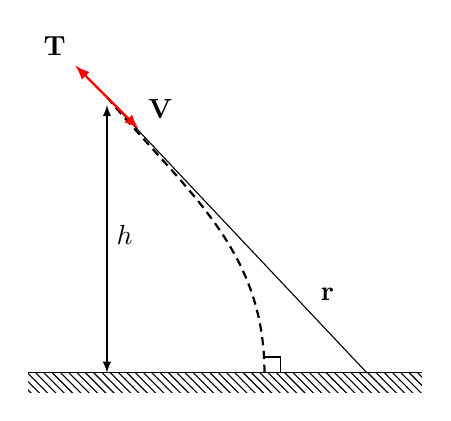
\begin{tikzpicture}[node distance={1.0cm and 1.0cm},>=latex]
        \draw (-1,0) -- (4,0);
        \draw (0,3.5) -- (3.3,0);
        \draw[densely dashed, thick] (0,3.5) to [out=-50, in =90] (2,0);
        \draw[<->] (0,0) -- (0,3.4);
        \draw[->, red, thick] (0,3.5) -- (0.4,3.1);
        \draw (0.4,3.1)node[rotate=0, anchor=south west] {$\mathbf{V}$};
        \draw[->, red, thick] (0,3.5) -- (-0.4,3.9);
        \draw (-0.4,3.9)node[rotate=0, anchor=south east] {$\mathbf{T}$};
        \draw (0, 3.5) node[] {\centerofmass}; 
        \draw (0,1.75)node[rotate=0, anchor=west] {$h$};
        \draw (2.8,1)node[rotate=0] {$\mathbf{r}$};
        \draw (2,0.2) -- (2.2,0.2) -- (2.2,0) ;
        \fill[pattern=north west lines] (-1,-0.25) rectangle (4,0); 
    \end{tikzpicture}
    \caption{Illustration of the flight profile for a gravity turn.}
    \label{fig:gravityturn}
\end{figure}

Given initial conditions, the law amounts to solving the following quadratic
equation for the acceleration $a$ to end up with zero velocity on the
surface:\cite{Citron1964}
\begin{align}
	\frac{a^2}{g^2}+ \sin\gamma_0 \left(\frac{v_0^2}{2h_0g}+1\right)
	\frac{a}{g} - \frac{\cos^2\gamma_0}{4v_0^2h_0g}
	\left(v_0^2+2gh_0\right)^2 \left(1 - \frac{v_0^2}{2rg}\right)=0
    \label{eq:gravt}
\end{align}
where $\gamma_0$ is the initial flight-path angle. Solving for $a$, the
commanded acceleration vector is then:
\begin{align}
    \mathbf{a}_c = -a \frac{\mathbf{v}}{v}
\end{align}
This simple law will null all velocity by the moment it arrives vertically on
the surface.

A strength of the classical gravity turn is its efficiency. Sostaric and Rea
(2005) show that it can indeed be more propellant-optimal than an Apollo-like
approach.\cite{Sostaric2005} However, rather than having a main braking and an
approach phase (with potentially different guidance laws), the gravity turn is
carried out on its own, starting from the pericenter of a Hohmann ellipse. Rea
(2009) points out that ``[while] the gravity turn may be near fuel-optimal for
descent from orbit, it is not a fuel optimal maneuver for target-redesignations
near the end of the terminal descent trajectory.''\cite{Rea2009} An approach
phase can hardly be combined with a gravity turn.

Eq.~\ref{eq:gravt} shows that the acceleration profile $a(t)$ is entirely dependent
on the initial conditions, and no feedback term is present. This limits the
achievable landing precision: would the spacecraft overshoot the planned
burn-initiation point, it could not target the planned landing-site anymore.

To correct for some of these deficiencies, Chomel and Bishop (2009) developed an
analytical algorithm, assuming a constant thrust-to-mass ratio over discrete
intervals, constant gravity, and no disturbing forces.\cite{Chomel2009} This
works by generating a reference trajectory, that is then followed by a
controller. Problematic about this method is that the generated trajectory is
two-dimensional. Although Chomel and Bishop say that cross-track retargetings
are possible, this can only be achieved through the controller. The method will
also be less computationally efficient than the original gravity turn, because
the analytical solution is highly nonlinear and contains dozens of
transcendental functions. The algorithm also failed in some cases, leading to
inefficient trajectories. Given the different landing architecture with lack of
an approach phase, Rea (2009) remarks that ``it may not be applicable to all
terminal descent situations, such as those with hazard avoidance maneuvers near
the end of the trajectory.''\cite{Rea2009} Path and thrust constraints are not
taken into account explicitly, and the mathematics do not allow for modification
to account for this. By eye-ball inspection of the plots given in the paper,
however, the viewing angle would seem to change only marginally and the
algorithm might thus be suitable from this perspective.

\subsection{Explicit Methods}

Explicit methods generate acceleration profiles based on the vehicle's state.
They provide closed-form expression derived analytically, and are thus
computationally efficient. However, necessary assumptions, difficulties in
considering constraints, and often involved mathematics can render explicit
methods sub-optimal in terms of propellant consumption and difficult to grasp.
These not being the only trade criteria for selecting guidance algorithms, however,
explicit methods are nevertheless very promising candidates.


\subsubsection{E-Guidance}
\label{sec:eguidancepreview}

$E$-Guidance and its variations form an influential group of gui\-dance
\-me\-thods for planetary landings. It was first proposed by Cherry (1964) and
later modified and extended by many.\cite{Cherry1964} $E$-Guidance is an
explicit guidance algorithm that solves the TPBVP, resulting in an analytical
equation. It is a very simple method, that can compute the trajectory in-flight.
To solve the TPBVP, an acceleration profile including gravity and thrust is
predefined as an integrable function.  This is done for each axis separately, by
example of the $x$-axis:\cite{Cherry1964a} 
\begin{align}
	\ddot{x}(t) &= c_1 + c_2 \tgo \\
	\begin{pmatrix}
	c_1 \\ c_2
	\end{pmatrix}
    &= \begin{bmatrix*}[r]
		 4/\tgo    & -6/\tgo^2\\
		-6/\tgo^2  & 12/\tgo^3
	  \end{bmatrix*}
	  \begin{pmatrix}
	  	\dot{x}_f - \dot{x}(t)\\
	  	x_f  - (x(t) + \dot x(t) \tgo)	  	
	  \end{pmatrix} \label{eqn:egcoeffs}
\end{align}
where \tgo is the time-to-go, or the time needed from the instantaneous location
to the target $\tgo=t_f - t$. The time-to-go has to be introduced because the
system is underdetermined and there are not sufficiently many equations to also
compute it along with $c_1$ and $c_2$. \tgo has to be established by other
means, such as an optimization.

The acceleration $\ddot{x}$ described by the polynomial with these coefficients
enforces a linear profile on the \emph{total acceleration} of the vehicle,
\emph{including gravity}. The thrust acceleration to be provided
by the propulsive plant in $x$-direction can be resolved simply by subtracting
this term as follows:
\begin{align}
	a_{T_x}(t) = c_1 + c_2 \tgo - g_x(t) \label{eqn:egaccel}
\end{align}

Although Cherry claims his method optimizes the functional
\begin{align}
    \minimize J = \int_{t_0}^{t_f} \sqrt{\transpose{\mathbf{a}_T} \mathbf{a}_T}\, \ed t
\end{align}
where $\mathbf{a}_T$ is the thrust acceleration (the acceleration without
gravity), this is not proven in his paper. Rather, it was later shown by
Ohlmeyer (2003), that $E$-Guidance does in fact optimize:\cite{Ohlmeyer2003}
\begin{align}
    \minimize J = \int_{t_0}^{t_f} \transpose{\mathbf{a}_T} \mathbf{a}_T\, \ed t
\end{align}
Unfortunately, the cost functions are not equivalent. The latter optimizes the
square of the thrust acceleration, and thus indeed minimizes the control effort,
but it \emph{does not minimize} the propellant
expenditure.\cite{Rea2009,Lion1971} This is only found by optimizing the
integral of the magnitude of the thrust. It could not be resolved from the
literature how large the difference between the two cost functions would be.
Rea (2009) calls guidance laws derived using this cost function ``near
fuel-optimal,'' hinting at relatively small differences.\cite{Rea2009}

$E$-Guidance is an adaptive algorithm that allows to target a new landing site
during the flight. However, the mathematics render a direct integration of any
constraints impossible---neither the viewing angle nor the thrust are
limited. This can lead to infeasible trajectories. It is still possible that
the generated trajectories meet the constraints, but this is not guaranteed. The
delivery to AG could be tailored to such conditions that generated trajectories
will be HDA compatible, although not with great robustness.


\subsubsection{Apollo Guidance}
\label{sec:apolloguidance}

The Apollo guidance system is an adapted version of $E$-Guidance and was flown
on six successful Lunar landings, making it the landing algorithm with the
strongest heritage. A similar profile was also chosen for future American lunar
landings and MSL.\cite{Paschall2009,Wong2006} The Apollo GNC system is described
in detail in Ref.~\citen{Klumpp1971}.

Compared to plain $E$-Guidance, the boundary conditions in Apollo guidance do
not only constrain the final position and velocity, but also the final
acceleration (and thus the attitude). The Apollo guidance equation is given
by:\cite{Bennett1970}
\begin{align}
\begin{split}
    \mathbf{a}(t) = & \left[3 \left(\frac{t_p}{\tgo}\right)^2
	                 -2 \left(\frac{t_p}{\tgo}\right)
	            \right]
	             \frac{12}{\tgo^2} (\mathbf{r}_f - \mathbf{r}) +
	            \left[4 \left(\frac{t_p}{\tgo}\right)^2
	                 -3 \left(\frac{t_p}{\tgo}\right)
	            \right]
	             \frac{6}{\tgo} \mathbf{v}_f \\ 
	             & +
	            \left[2 \left(\frac{t_p}{\tgo}\right)^2
	                 -  \left(\frac{t_p}{\tgo}\right)
	            \right]
	            \frac{6}{\tgo} \mathbf{v} +
	            \left[6 \left(\frac{t_p}{\tgo}\right)^2
	                 -6 \left(\frac{t_p}{\tgo}\right) + 1
	            \right] \mathbf{a}_f
\end{split}
\end{align}
In this equation $t_p$ is the time adjusted for computer lag, $t_p = \tgo +
t_l$, where $t_l$ is the lag. The lag could amount to \SI{2.5}{s} in the
1960s,\cite{Klumpp1971} but is ignorable today, so one may set $t_l =
\SI{0}{s}$ and thus $t_p/\tgo=1$.

Because the final thrust vector can be taken into account in Apollo guidance,
the trajectory can be tuned to suit the instruments' FOV better.
Nevertheless, constraints cannot be taken into account explicitly. Retargetings
are easily feasible due to the low computational load, but the lack of thrust
bounds can be problematic.

\subsubsection{Modified Apollo Techniques}

As mentioned before, the Apollo (or $E$-) guidance principle is the
most-widespread landing guidance mode. This is illustrated by the large number
of papers applying this method. Some of the more recent ones are:
Refs.~\citen{Sostaric2005,Steinfeldt2008,Delaune2010,Carman1998,Lafontaine2004,
    Sostaric2007}. The principle is always the same. One assumes an acceleration
profile of either linear, quadratic, or cubic order, such as:
\begin{align}
	a_x = c_1 + c_2 t + c_3 t^2
\end{align}
This is then either integrated to obtain a modified $E$-matrix formulation, or
optimized using a numerical method. When a quadratic profile is chosen, such as
above, this yields a very popular kind of trajectory called ``quartic
guidance'', as the trajectory will be a fourth-order polynomial. The method is
intriguing, because it is so simple and gives insight into the problem.  
Even in modified methods, for example, it will never be possible to take into
account constraints explicitly. However, modified algorithms might yield a trajectory 
that is more suitable for HDA than the classic algorithm.


\subsubsection{Explicit Mode with Weighting on Final Time}

D'Souza derived an algorithm that is derived from optimal control
theory,\cite{Bryson1975} and thus explicitly optimal.\cite{DSouza1997} The
author makes several assumptions: flat, non-rotating, atmosphereless body, and
constant, vertical gravity. The quadratic performance index is then specified
as:
\begin{align}
	\min J = \Gamma t_f + \frac{1}{2} \int_{t_0}^{t_f} 
    \transpose{\mathbf{a}_T} \mathbf{a}_T \, \ed t
\end{align}
where $\Gamma$ is a weighting on the final time, which can be used to adjust the
trajectory. Note that as for $E$-Guidance, only the square of the acceleration
is optimized, which is not equivalent to minimizing the propellant expenditure.
It is near propellant-optimal, however.  Using the calculus of variations, it
can be shown that the optimal control accelerations are:
\begin{align}
	\mathbf{a}_T = -4 \frac{\mathbf{v}}{\tgo}
	             -6 \frac{\Delta \mathbf{r}}{\tgo^2}
	             -\mathbf{g}
\end{align}
where $\Delta \mathbf{r} = \mathbf{r} - \mathbf{r}_f$ and $\mathbf{g} =
\transpose{\left(\begin{matrix} 0 & 0 & g \end{matrix}\right)} = \const$ There is no
$\Delta \mathbf{v}$ because the final velocity is assumed to be $\mathbf{v}_f =
\mathbf{0}$.

A favourable feature of D'Souza's mode is that the optimal time-to-go can be
solved directly using a quartic equation. There is thus no need for iteration,
numerical optimization, or other ways of estimating a suitable \tgo.
The equation to be solved is:
\begin{align}
    \left(\Gamma + \frac{g^2}{2}\right) \tgo^4 - 2\transpose{\mathbf{v}}\mathbf{v}
    \tgo^2 - 12 \transpose{\mathbf{v}}\mathbf{r} - \tgo - 18 \transpose{\mathbf{r}}
	\mathbf{r} = 0
\end{align}
for which an analytical solution is provided in the paper.
The method is thus an explicit, three-dimensional guidance mode. Necessary
and sufficient optimality conditions are fulfilled as well. 

One limitation is that no constraints are taken into account. It can thus happen
that subterranean trajectories are generated. This can be overcome by changing
the weighting factor $\Gamma$ and propagating the trajectory to check its
validity, at added computational cost. This was tested in
Ref.~\citen{Steinfeldt2008} and found to be simple to implement and still
computationally less demanding than other guidance modes. Another limitation is
that it is implicitly assumed that $\mathbf{v}_f = \mathbf{0}$. This might cause
trouble with some landing architectures. If a constant-speed terminal
vertical-descent is planned, for example, delivery to TG could be
required to be at finite vertical velocity.

For this guidance mode, it could be possible to harness $\Gamma$ as a tuning
parameter, and tune it such that resulting trajectories are more HDA-suitable.
This is untested as of yet. The law is fully adaptive and can accommodate
retargetings. Again, $\Gamma$ might also be used to increase the time-of-flight
to give more time for retargeting and HDA surveying, trading flight time for
propellant. Constraints cannot be taken into account explicitly, however.

\subsection{Numerical Methods}
\label{sec:numerical}

Numerical methods often solve similar problem formulations as explicit methods,
but can do so with less simplifications and while enforcing constraints. This
makes such guidance algorithms very robust and propellant-efficient, while
coming at the cost of computational expense. However, recent advances in
optimization theory have led to dramatic increases in the numerical efficiency,
making numerical methods compelling upcoming candidates for on-board guidance.
Ever more powerful on-board computers also make the future application of such
methods more likely.


\subsubsection{Convex Guidance}

\providecommand{\norm}[1]{\lVert#1\rVert}


Recently, Açıkmeşe and Ploen (2007) published a promising guidance mode based on
convex optimization theory.\cite{Acikmese2007,Boyd2004}  If a problem turns out
to be convex, or can be rewritten as a convex problem, the optimization becomes
easier and can be solved efficiently.  They formulate the guidance problem as a
second-order cone problem (SOCP), which makes it very computationally efficient
for a numerical algorithm.\cite{Lobo1998} Convex optimization has received lots
of attention in the past decade, and Açıkmeşe and Ploen are the first to publish
an application to the guidance problem. In fact, the algorithm was designed for
actual flight implementation from the start.

Convex optimization is a field that is involved and abstract. A detailed
discussion of the algorithm is beyond the scope of this paper. Some
distinguishing remarks can still be made:
\begin{itemize}
    \item Convex optimization theory proofs that a well-posed convex problem
          (which this is) is \emph{guaranteed} to converge.
    \item It can also be shown that the obtained solution will be the
          \emph{global} optimum.
    \item There are a number of different, very efficient solvers for this kind
          of problem. The authors apply an interior-point method.  These can be
          provided ``with a deterministic stopping criteria [\emph{sic.}], and
          with prescribed level of accuracy'' .\cite{Acikmese2007}
    \item The performance index is $J = \int \norm{\mathbf{T}} \ed t$, and
          thus truly propellant-optimal, in contrast to $E$-Guidance, for
          example.
    \item Constraints and penalties can be imposed.
    \item Assumptions for the problem formulation: constant vertical gravity, no
          other disturbing forces.
\end{itemize} 

Figure~\ref{fig:socpthrust} shows that  the previously stressed
\emph{max-min-max} trajectory that was discussed in
Section~III.\ref{sec:observations} is in fact commanded. Here, the engines cannot be
turned off entirely, and are thus throttled to the lowest possible setting. This
is an indication that this guidance mode truly finds the global optimum, as
claimed by the authors.

\begin{figure}
    \centering
    \includegraphics[width=0.4\textwidth]{ThrottleSOCP.pdf}
    \caption{%
        Thrust profile for a Mars descent as computed by convex guidance. 
        Source: Ref.~\citen{Acikmese2007}
    }
    \label{fig:socpthrust}
\end{figure}


The main advantage of this guidance mode is that it has been designed for
on-board implementation right from the beginning on. Putting the problem as an
SOCP makes it very efficiently solvable. It can also take constraints into
account, such as altitude limits (to avoid subterranean trajectories), or thrust
limits. Moreover, it is advantageous for validation that the algorithm is proven
to be optimally convergent. Retargetings are possible, although the
re-computation of the trajectory for a diversion will take more time than with
other modes.

\subsubsection{Gradient-based Optimization}

Although computationally expensive, classical numerical optimization techniques
can also be applied to solve the guidance problem.  Steinfeldt et al.\ (2008)
applied a gradient-based numerical optimization-technique to the guidance
problem.\cite{Steinfeldt2008}  Gradient-based techniques are
essentially a computational implementation of optimal control theory. For more
details, see Ref.~\citen{Bryson1975}.

The cost-function specified by the authors is:
\begin{align}
    \text{minimize\ } J = \int_{t_0}^{t_f} \transpose{\mathbf{a}_T}\mathbf{a}_T \,
    \ed t 
\end{align}
so there is no penalty on any final conditions. Although coming at a
computational expense, gradient-based methods can take constraints into account,
such as a thrust limit or altitude restriction, and also viewing angles. The
gradient-based mode will also result in optimal trajectories, saving in
propellant mass.\footnote{Steinfeldt et al.\ most likely chose the sub-optimal
    performance criterion shown above for reasons of comparability to the
    explicit guidance mode formulated by D'Souza,\cite{DSouza1997} and it would
    have been possible to use more optimal one using a gradient-based
    optimizer.}

The biggest disadvantage is that the method is extremely computationally
intensive (see Ref.~\citen{Steinfeldt2008}). The method has also not been
analyzed with respect to hazard avoidance in any published work. On the one
hand, it shows great promise, because a viewing angle can be either put under
penalty or even enforced in this method. On the other hand, possibly long
execution times on space-grade computers could hinder retargetings, because it
needs too much time to calculate the guidance command.


\subsubsection{Neural Guidance}

\noindent An innovative approach to spacecraft guidance is to train an
artificial neural network (ANN). This was first published by Gelly and Vernis
(2009).\cite{Gelly2009}. ANNs are applied to many different domains, especially
in control engineering.\cite{Haykin1998} Networks can be trained by using models
and sets of constraints and boundaries. The method by Gelly and Vernis chooses a
heuristic approach, where neurons are trained by \num{600} generations of a
genetic algorithm using a full set of equations of motion. Solutions that do not
meet the constraints are penalized, leading to a ``quasi-constrained'' guidance
algorithm. The result is a numerical input-output relation that can act as a
guidance law. The network used for guidance is shown in
Figure~\ref{fig:neuralnetwork}.

\begin{figure}
	\centering
	\includegraphics[width=0.6\textwidth]{NeuralNetwork.png}
	\caption{Neural network used for spacecraft guidance in
        Ref.~\citen{Gelly2009}.}\label{fig:neuralnetwork}
\end{figure}

A major strength of this method is that it allows to cope with problems that do
not have an analytical solution. This means that for the landing guidance
problem, less simplifications have to be made. For example, no constant gravity
needs to be assumed. 

The biggest problem is that no insight is gained, neither in the problem, nor in
the outcome. The ANN acts as a black-box, which generates a solution.  This
makes it very difficult to validate for real missions. It cannot be proven that
the guidance mode is convergent.  While the authors claim they generated a very
robust scheme by training the network under broad dispersions, further
investigation would be necessary. The possibility of quasi-constraining the mode
makes the approach favourable for HDA. Gelly and Vernis confirmed that the
algorithm is capable of successfully diverting to a new target. Still, the
constraints are not enforced, and convergence is not guaranteed, so the
validation problem remains.

% \lettrine{F}{our} algorithms that can potentially work in an \ac{acr:hda}
% framework have been identified from the literature. These can be divided into
% two groups: explicit and numerical algorithms. From the survey it can be
% concluded that it is currently not possible for explicit algorithms to taken
% into account landing-site viewing-angle constraints. Numerical algorithms, can
% either truly enforce constraints in an optimization (convex guidance), or
% penalize solutions that do not meet constraints (neural guidance). Nevertheless,
% the boundary conditions can be tuned to achieve feasible trajectories
% with explicit guidance laws as well, as was done for Apollo. All algorithms are
% adaptive and can re-generate trajectories for diverts on-board. Explicit
% algorithms can adapt faster because they are much simpler, being based on
% closed-form expressions rather than iterative routines.
% 
% Some of the laws have been analyzed in trade-offs before
% \autocite{Sostaric2005,Steinfeldt2008}. These papers confirm that retargetings
% are possible, but could do not provide a full guidance analysis in scope of
% \ac{acr:hda} \ac{acr:gnc} systems. This is also the major limitation of this
% paper. As no common test cases have been run for all algorithms, no final
% conclusion on the suitability of algorithms can be drawn. There is thus
% outstanding research potential to find the guidance algorithm that is
% best-suited for such systems.

\subsection{Other Methods}

The algorithms shown in the previous sections form a pre-selected set of
promising candidates for guidance algorithms that need to operate in constrained
landing environments. However, many more algorithms have been published, but
were not discussed in further detail for several reasons, such as immaturity or
the lack of 3D terminal-state-vector control, or simply because time did not
permit their detailed study. For completeness' sake of the literature survey,
they are still be mentioned here.

Braking phases usually use the optimal bi-linear tangent steering
law.\cite{Lawden1963} However, it cannot be used to directly target a final
state. The Space Shuttle used a derived variant called powered explicit guidance
(PEG), which is, however, not able to constrain the downrange
position.\cite{McHenry1979} An extension of the PEG to full
terminal-state-vector control was later developed, but remains unpublished and
never flew on the shuttle.\cite{Rea2009,Fill1989} Najson and Mease have developed
a computationally inexpensive algorithm based on closed-form expressions derived
from optimal control theory. It solves simplified sub-problems with sub-optimal
performance criteria.\cite{Najson2006} Ueno and Yamaguchi present a law that was
initially proposed for the SELENE mission, but that cannot constrain down- and
crossrange.\cite{Ueno1999} Uchiyama derived a law using a barrier-function
method, which is sub-optimal and unconstrained in the thrust. It generates a
reference trajectory that is then tracked by a controller.\cite{Uchiyama2007}
Flatness theory has been applied to the guidance problem by Desiderio and
Lovera. This results in a two-dimensional trajectory that is tracked by a
controller.\cite{Desiderio2012} Another two-dimensional law with heritage of the
bi-linear tangent steering has been proposed by Lee.\cite{Lee2011} For missions
with a sequential engine shutdown rather than throttleable engines, Springmann
et al.\ present a guidance algorithm that targets a downrange component by timed
shutdowns. However, this leads to considerable landing
errors.\cite{Springmann2006} Horn showed the application of a 2D iterative law
with heritage of bi-linear tangent steering.\cite{Horn1965,Horn1965a} Lunghi et
al.\ combined a classical explicit algorithm with modern optimization techniques
to impose constraints.\cite{Lunghi2013} Rea and Bishop reduced the
dimensionality of the landing problem, assuming constant thrust and a free
time-of-flight.\cite{Rea2010}

Some of the guidance laws have been compared in a trade-off in
Ref.~\citen{Steinfeldt2008}. It is pointed out that the above is merely a
literature review, and can only form the basis for a trade-off inasmuch it is
used as the starting point for identifying first candidates. A consolidated trade
method for guidance algorithms is proposed in Ref.~\citen{Steinfeldt2010}.


\section{Unconstrained Explicit Algorithm}

The previous sections have rigorously introduced the state-of-the-art in
approach-phase guidance algorithms, starting with the description of a reference
scenario, putting the guidance modes into context by describing key technologies
for next-generation landers, and finally defining an overarching mathematical
problem. To round it off, this section gives an example for an algorithm:
$E$-Guidance, an explicit, unconstrained guidance mode (see
Section~IV.\ref{sec:eguidancepreview}).

The choice for $E$-Guidance can be motivated by its wide-spread use, simplicity,
and ease of implementation---this makes it the perfect candidate for a reference
algorithm in trade studies (\eg, Ref.~\citen{Sostaric2005}). The
following test-cases can serve as a reference for verification of future studies,
or a base for comparison to other algorithms.



\subsection{Description of the Algorithm}

The $E$-Guidance law is based
on constraining the vehicle's \emph{total} acceleration profile, including thrust
acceleration \emph{and gravitational acceleration}, to be a linear polynomial with time.
This total constrained acceleration $\mathbf{a}$ can be written as:
\begin{align}
    \mathbf{a}(t)=\mathbf{a_c}+\mathbf{g} = \mathbf{c}_1 + \mathbf{c}_2(t_f-t) 
                 =\mathbf{c}_1 + \mathbf{c}_2  \tgo
        \label{eqn:totalaccel}
\end{align}
where $\mathbf{a}_c$ is the acceleration command that the guidance system will
generate, to be realized by the spacecraft's propulsion unit, and $t$ and $t_f$
are the current and final time at landing, respectively. The two real (ideally
constant) vectors $\mathbf{c}_1$ and $\mathbf{c}_2$ and the time-to-go $\tgo$
can be computed to shape the profile such that it satisfies the initial and
final boundary conditions. The derivation starts with the
Eq.~(\ref{eqn:totalaccel}) by integration in time, which results in analytic
solutions for the velocity and trajectory.  For all practical purposes in
guidance, however, the thrust acceleration command and not the total
acceleration is required. This is found simply by subtracting $\mathbf{g}$ from:
\begin{align}
    \mathbf{a}_c = \mathbf{a} - \mathbf{g} = \mathbf{c}_1 + \mathbf{c}_2 \tgo- \mathbf{g}
    \label{eq:thrustcommand}
\end{align}

Integrating Eq.~\eqref{eqn:totalaccel} twice yields the following matrix equation, which
is a closed-form solution for the coefficients (leaving $\tgo$ free):
\begin{align}
    \begin{pmatrix}
	\mathbf{c}_1\\ \mathbf{c}_2
    \end{pmatrix} =
    \begin{bmatrix}
	-\frac{2}{\tgo}   &  \frac{6}{\tgo^2}\\
	 \frac{6}{\tgo^2} & -\frac{12}{\tgo^3}\\
    \end{bmatrix}
    \begin{pmatrix}
	\mathbf{v}_f - \mathbf{v}_0\\
	\mathbf{r}_f - \mathbf{r}_0 - \mathbf{v}_0 \tgo
    \end{pmatrix}
    \label{eq:coefficients}
\end{align}
This equation shows that the accelerations $\mathbf{a}_0$ and $\mathbf{a}_f$
are not taken into account as boundary conditions and thus instantaneous changes
of thrust magnitude and attitude will occur when $E$-Guidance is first executed.
This is disregarded in this 3-DOF simulation.

A note of caution is required because $(\mathbf{c}_1, \mathbf{c}_2) \to \infty$
as $\tgo\to0$, as the time-to-go is in the denominator of the fractions in the
matrix. According to Eq.~\eqref{eq:thrustcommand} this will lead to an
infinite thrust command as the vehicle comes very close to the landing site.
This issue is circumvented by stopping to recompute the coefficients after
$\tgo\leq \SI{1}{\second}$.

The time-to-go remains a free parameter. In Eq.~\eqref{eq:coefficients},
\tgo may thus be freely specified, and $\mathbf{c}_1$ and $\mathbf{c}_2$
will then be computed such that the acceleration profile will steer the
spacecraft from the initial conditions to the final conditions within this time.
This also disregards any constraints: it can happen that the thrust commanded is
higher than the engine capacity. The designer must be aware of this limitation
and resolve it by specifying suitable initial conditions, and possibly
restricting diversion maneuvers. 

Many methods exist for determining the time-to-go. Some are covered in
Refs.~\citen{Steinfeldt2008,Wong2006,Cherry1964a,Klumpp1971,Lafontaine2004,DSouza1997},
comprising methods for $E$-Guidance and other explicit algorithms. The proposed
method presented here is based on solving the rocket equation. Comparisons to
numerical optimizations with \tgo as independent variable show that this method
approaches the propellant optimum.  This method is, in fact, a modification of
the method described in Ref.~\citen{Cherry1964a}. In this paper, Cherry
describes a method to determine a time-to-go for a \emph{fixed}-thrust rocket.
The propulsion configuration considered in this paper assumes a throttleable
propulsion device, and thus Cherry's method needs to be adapted.

Starting by assuming a fixed-thrust rocket, the final vehicle mass $m_f$ after a
certain burn time $t_b$ will be:
\begin{align}
    m_f = m_0 - \dot{m}_c t_b 
        \label{eq:masses}
\end{align}
where $\dot{m}_c$ is the constant mass-flow rate of the engine. The time-to-go
was previously defined as
\begin{align*}
    \tgo = t_f - t    
\end{align*}
If it is assumed that time starts running at \SI{0}{\second}, then the engine
will still burn for as long as the time-to-go, and thus the two are identical:
\begin{align}
    t_{b} = \tgo
\end{align}

The rocket equation reads:
\begin{align}
    m_f = m_0 e^{-\Delta V / V_e}
        \label{eq:rocketeq}
\end{align}
Combining Eqs.~\eqref{eq:masses} and \eqref{eq:rocketeq}:
\begin{align}
    m_0 - \dot{m}_c t_{go} = m_0 e^{-\Delta V/V_e}
\end{align}

The characteristic time is now introduced. This quantity represents the
time it would need to burn up the entire vehicle were it made up only of
propellant and the mass flow be constant:
\begin{align}
    \tau = \frac{m_0}{\dot{m}_c}
\end{align}
Combining the two previous equations and rearranging gives:
\begin{align}
    \tgo = \tau \left( 1 - e^{-\Delta V/V_e} \right)
        \label{eq:tgofixedt}
\end{align}
This equation allows to compute \tgo for a fixed-thrust rocket for a given
$\Delta V$ and assuming perfectly fixed thrust. When applying the formula to a
variable-thrust rocket, however, the estimation is unstable because of the
dependency on the mass-flow. With every iteration, the time-to-go will become
shorter because the thrust, and hence mass-flow, will go up.  To avoid this,
$\tau$ is redefined as follows:
\begin{align}
    \tau = \tau_0 - t 
\end{align}
where $\tau_0$ is the initial value obtained at the first iteration after the
initialization, and $t$ is the time running from \SI{0}{\second} onwards at the
first call of the guidance law. Note that this is essentially a scaling with
respect to the current vehicle mass assuming constant mass flow:
\begin{align}
    \tau = \tau_0 - t \quad \Leftrightarrow \quad \tau = \frac{m_0}{\dot{m}} - t \quad \Leftrightarrow \quad \tau = \frac{m_0 - \dot{m} t}{\dot{m}} = \frac{m}{\dot{m}}
\end{align}
$\Delta V$ is easily computed including gravity losses:
\begin{align}
    \Delta V = \sqrt{(\dot{x} - \dot{x}_f)^2 + (\dot{y} - \dot{y}_f)^2 +
        (\dot{z} - \dot{z}_f + g \tgo)^2}
\end{align}


$\tau$ has to be initialized with $\tau_0$ as the following value:\footnote{The
    quantity $\tau = m/\dot{m}$ is commonly encountered and is also called
    the characteristic time. It can be interpreted as the time it would take to
    burn up the entire vehicle, were it made up only of propellant and the mass
    flow rate constant.}
\begin{align}
    \tau_0 = \frac{m_0}{\dot m} 
\end{align}
where $m_0$ is the initial spacecraft mass and $\dot{m}$ is the engine's
mass-flow. The latter equation is dependent on the mass-flow rate, which
constitutes a problem for guidance as shown next. Rewriting the equation:
\begin{align}
    T(t_0) = m_0 a_c = \dot{m} V_e \quad \Leftrightarrow \quad \frac{m_0}{\dot{m}}
    = \frac{V_e}{a_c} = \tau_0 
\end{align}
This illustrates how $\tau_0$ is dependent on the commanded acceleration---a
quantity that is to be computed by guidance and thus clearly not known at the
first time step. For this reason, the time-to-go first has to be initialized
differently, after which the resulting thrust acceleration may be used to
compute $\tau_0$ and the primary procedure described above can be used. 

The way how this is initialized is not very important, because the primary
method will converge to a steady value very quickly. Test runs have shown that
the following value results in a good first estimate that will not be too far
from what the primary method will determine:
\begin{align}
    \tgo = 2\frac{x_f-x}{\dot{x}_f - \dot{x}} \Bigg|_{\text{along track}} 
\end{align}
where all quantities must be given in the along-track direction, such that the
position vector of the spacecraft is in the $x$-$y$ plane of the coordinate
system ($x$ along track, $y$ cross track, $z$ completes the triad). The switch
from this initialisation method to the primary estimation technique occurs after
a user-specified time. 


\subsection{Simulation Results}

Two different test cases have been investigated to demonstrate the applicability
of $E$-Guidance to different scenarios. First, the landing of a light Mercury
lander approaching at high velocity has been simulated. This is the scenario
that has originally been investigated for a hermian surface element of the
Bepi Colombo mission.\cite{Novara2002} Second, the approach
phase of the ESA Lunar Lander as described in Section~II.A.\ has been tested. 

Table~\ref{tab:ICs} lists the boundary conditions applied in the simulations. In
case of the Mercury landing, the guided descent starts at about \SI{20}{km}
downrange at an altitude of \SI{8.3}{km}. The vehicle is approaching very fast
at \SI{753}{m/s}. The target in this case is the landing site, which is placed
at the origin of the reference frame. Note that because this variant of
$E$-Guidance cannot constrain the final acceleration, the boundary conditions
are only substantiated by position and velocity vectors. The lunar test case
starts at only \SI{1.6}{km} downrange and altitude with respect to the landing
site. The heavier vehicle approaches at about \SI{155}{m/s}, and is thus much
slower than the Mercury lander during its descent. Following the mission
scenario of Section~II.A., the target is TG at \SI{15}{m} altitude above the
landing site, from which a \SI{1.5}{m/s} vertical descent is to be flown down to
the surface.

\begin{table}[htb]
    \centering
    \small
    \caption{Initial and final boundary conditions for the 2D simulation. Origin at landing site.}
        \label{tab:ICs}
    \centerline{%
    \begin{tabular}{lcrr}
        \toprule
                    &           & \multicolumn{2}{c}{Magnitude} \\ \cmidrule(lr){3-4}
        Quantity    & Symbol    & \multicolumn{1}{c}{Mercury} & \multicolumn{1}{c}{Moon}\\
        \midrule
        Initial downrange position, m & $x_0$     & $-\num{20169}$ & $-\num{1601}$ \\
        Initial altitude, m           & $y_0$     & \num{8377}     & \num{1569}    \\
        Initial downrange speed, m/s  & $v_{x_0}$ & \num{712.61}   & \num{150}     \\
        Initial descent rate, m/s & $v_{y_0}$ & $-\num{242.36}$ & $-\num{40}$\\
        \midrule
        Final downrange position, m & $x_f$     & \num{0} & \num{0}   \\
        Final altitude, m           & $y_f$     & \num{0} & \num{15}  \\
        Final downrange speed, m/s  & $v_{x_f}$ & \num{0} & \num{0}   \\
        Final descent rate, m/s   & $v_{y_f}$ & \num{0} & $-\num{1.5}$ \\
        \midrule
        Initial mass, \si{\kilo\gram}   & $m_0$ & \num{450} & \num{760}\\
        Engine's specific impulse, \si{\second} & $I_{sp}$  & \num{315} & \num{325}\\
        \bottomrule
    \end{tabular}}
\end{table}

To allow for the reproducibility of the results, the simulation parameters for
both test cases are shown in Table~\ref{tab:params}. All simulations have been
performed in a Matlab/Simulink test bed. The equations of motion have been
restricted to the three translation degrees of freedom.

\begin{table}[htb]
    \centering
    \small
    \caption{Simulation parameters.}
        \label{tab:params}
    \begin{tabular}{lcrr}
        \toprule
                    &           & \multicolumn{2}{c}{Magnitude} \\ \cmidrule(lr){3-4}
        Quantity    & Symbol    & \multicolumn{1}{c}{Mercury} &
        \multicolumn{1}{c}{Moon}\\
        \midrule
        Planetary radius, \si{\meter} & $R$ & \num{2439870} & \num{1738000} \\
        Gravitational
        parameter, \si{\meter\cubed\per\square\second\per\kilo\gram}   & $\mu$ & \num{22.030944e12} & \num{4.902801076e12} \\
        Rotational speed, \si{\radian\per\second} & $\omega$ & \num{1.2399e-6}& \num{2.6617073e-6}\\
        \midrule
        Standard gravitational acceleration, \si{\meter\per\second\square} & $g_0$  & \num{9.80665} & \num{9.80665}\\
        \midrule
        Runge-Kutta 4 integrator step size, \si{\second} & $\Delta t$    & \num{0.01} & \num{0.01} \\
        Maximum time-span, \si{\second} & $t_{max}$     & \num{100} & \num{100} \\
        \bottomrule
    \end{tabular}
\end{table}



\subsubsection{Mercury High-speed Approach}

The results for the hermian test case are shown in Figure~\ref{fig:mercury}.
The trajectory is plotted in Figure~\ref{fig:mercury}~(a), in which the
commanded acceleration vector is indicated as the blue arrow in ticks of
\SI{2}{s}, offers insight into the suitability of $E$-Guidance for HDA in this
scenario. Because of the high-speed approach, the trajectory has little
curvature and resembles a straight line. At the same time, the commanded
acceleration, which corresponds to the attitude of the spacecraft, hardly
changes direction, which can also be observed in Figure~\ref{fig:mercury}~(b).
Note that the pitch is measured from the vertical here, so that \ang{0}
describes an upright attitude with respect to the local horizontal. Such a
steady attitude is ideal for HDA because the landing site can easily be kept in
the FOV. Moreover, the circumstances are ideal for navigation cameras, their
orientation can remain almost ideal due to the small changes in pitch. Attitude
rates are also small, which reduces image smearing.

\begin{figure}
    \centering\small
    \null\hfill\subfloat[][Trajectory.]{
        \begin{tikzpicture}
            \begin{axis}[
                width=0.45\textwidth,
                height=0.2\textheight,
                grid,
                xlabel={downrange ($x$), km},
                ylabel={altitude ($y$), km},
                font=\small,%
                ]
                \addplot[red, no markers] table [x expr={-\thisrowno{0}},y
                expr={\thisrowno{2}}, col sep=comma] {Data-Mercury/radius.csv};
                \addplot[blue, quiver={u=-\thisrowno{2}, v=\thisrowno{3}, scale
                    arrows=0.1}, each nth point={200}, -stealth] table [col
                sep=comma]
                {Data-Mercury/accelerationquiver.csv};
            \end{axis}
        \end{tikzpicture}}\hfill\subfloat[][Pitch profile.]{\begin{tikzpicture}
            \begin{axis}[
                xmax=55,
                xmin=0,
                ytick={20,25,...,35},
                width=0.45\textwidth,
                height=0.2\textheight,
                grid,
                font=\small,%
                xlabel={time ($t$), s},
                ylabel={pitch ($\theta$), \si{\degree}},
                ]
                \addplot[red, no markers] table [x expr={\thisrowno{1}},y
                expr={90-\thisrowno{0}}, col sep=comma] {Data-Mercury/pitch.csv};
            \end{axis}
        \end{tikzpicture}}\hfill\null 
    
    \null\hfill\subfloat[][Thrust command.]{%
        \begin{tikzpicture}
            \begin{axis}[
                width=0.45\textwidth,
                height=0.2\textheight,
                grid,
                xmax=55,
                xmin=0,
                ymin=0,
                %ymax=450,
                ylabel={thrust ($T$), \si{\newton}},
                xlabel={time since AG ($t$), \si{\second}},
                font=\small,%
                legend pos=outer north east,%
                ]
                \addplot[red, no markers] table [x expr={\thisrowno{1}},y
                expr={\thisrowno{0}}, col sep=comma] {Data-Mercury/thrust.csv};
            \end{axis}
        \end{tikzpicture}}\hfill\subfloat[][Time-to-go estimation.]{\begin{tikzpicture}
            \begin{axis}[
                width=0.45\textwidth,
                height=0.2\textheight,
                grid,
                xmax=55,
                xmin=0,
                ymin=0,
                ylabel={time-to-go ($t_{go}$), \si{\second}},
                xlabel={time since AG ($t$), \si{\second}},
                font=\small,%
                ]
                \addplot[red, no markers] table [x expr={\thisrowno{1}},y
                expr={\thisrowno{0}}, col sep=comma] {Data-Mercury/timetogo.csv};
                \node[coordinate, pin={[align=center,font=\tiny,
                    pin edge=thick]-0:{$t_{go}$ switch-over}}]
                at (axis cs:0.3,49) {};
                \node[coordinate, pin={[align=center,font=\tiny,
                    pin edge=thick]-265.8:{$t_{go}$ threshold}}]
                at (axis cs:51.5,1) {};
            \end{axis}
        \end{tikzpicture}}\hfill\null 
    \caption{Simulation results of the hermian test-case. The blue arrows
        indicate the commanded acceleration in ticks of \SI{2}{s}. Pitch
        measured from the vertical.}
    \label{fig:mercury}
\end{figure}

The thrust profile is shown in Figure~\ref{fig:mercury}~(c). The peak in the
beginning occurs due to the initialization of the time-to-go (see previous
section), which can also be observed in Figure~\ref{fig:mercury}~(d). It can be
ignored if more realistic simulations are desired. The thrust command is clearly
increasing, calling for a throttleable engine. The results of the time-to-go
estimation are shown in Figure~\ref{fig:mercury}~(d). After the switch-over,
\tgo behaves almost linearly, which demonstrates the consistency of the method,
leading to a smooth approach. The final flat part of the graph indicates the
cut-off of the \tgo at \SI{1}{s} to avoid infinite thrust commands.

Although these results appear to be promising, they are not flawless. First, the
final attitude of the spacecraft at landing is inclined by \ang{37} with respect
to the local vertical. The spacecraft is thus landing at an oblique angle, which
is not acceptable. This problem results from the unconstrained final
acceleration vector. If an Apollo-like algorithm (quartic guidance) was applied,
this problem could be resolved---at the cost of a slightly higher complexity. It
would also be possible to adapt the mission scenario, or to tune the time-to-go
to achieve a more suitable attitude.

The landing does also not occur without any errors in speed and position. These
are shown in Table~\ref{tab:FCs}, which documents the achieved final conditions.
Whereas the landing site is reached almost without error, the velocity
components fail to be reduced to \SI{0}{m/s} exactly. However, even the maximum
error of about \SI{1}{m/s} in the downrange speed is tolerable for most landers.
Nevertheless, the impact of these errors must be further investigated,
considering that this simulation considers perfect navigation and control, and
errors can thus be expected to be larger in high-fidelity simulations.

\begin{table}
    \centering
    \small
    \caption{Achieved final conditions.}
        \label{tab:FCs}
    \centerline{%
    \begin{tabular}{lcrrrr}
        \toprule
                    &           & \multicolumn{2}{c}{Mercury} & \multicolumn{2}{c}{Moon} \\ \cmidrule(lr){3-4} \cmidrule(lr){5-6}
        Quantity    & Symbol    & \multicolumn{1}{c}{Magnitude} & \multicolumn{1}{c}{Error} & \multicolumn{1}{c}{Magnitude} & \multicolumn{1}{c}{Error} \\
        \midrule
        Achieved downrange position, m & $x_f$     & \num{2.14e-6} & --- & $-\num{0.03}$ &  \num{0.03} \\
        Achieved altitude, m           & $y_f$     & \num{2.77e-6} & --- & \num{14.99} &  \num{0.01} \\
        Achieved downrange speed, m/s  & $v_{x_f}$ & $\num{0.95}$  & \num{0.95} & $-\num{0.06}$ &  \num{0.06}  \\
        Achieved descent rate, m/s     & $v_{y_f}$ & $-\num{0.56}$ & \num{0.56} & $-\num{1.42}$ & \num{0.08}  \\
        \midrule
        Consumed propellant mass, \si{\kilo\gram}   & $m_p$ & \num{106.88} & --- & \num{53.01} & ---\\
        \bottomrule
    \end{tabular}}
\end{table}

\subsubsection{Moon Low-speed Approach}

Figure~\ref{fig:moonfail} shows the resulting trajectory for the lunar test case
if the guidance commands are computed with the $E$-Guidance method previously
presented. It is very obviously visible that the method has severe trouble in this case,
because the vehicle is actually first commanded to fly upside down and begins to accelerate
towards the landing site, only to pitch over again and brake towards the end. It
shall be noted that the guidance algorithm successfully achieves the final
boundary conditions with little error. Nevertheless, such a trajectory is
unfeasible in reality for several reasons.

This failed test indicates that the \tgo-estimation method derived in
Section~V.A.\ is not applicable without modification for the whole range of
mission scenarios. In this simulation, the cause of the problem is that the
speed is rather low, yielding a small $\Delta V$ and consequently a short
time-to-go. To reach the landing site ``in time'', the vehicle is thus
accelerated towards it, so it flies faster and arrives within the predicted
time-to-go.

\begin{figure}
    \centering\small
    \begin{tikzpicture}
        \begin{axis}[
            width=0.45\textwidth,
            height=0.3\textheight,
            grid,
            axis equal,
            xlabel={downrange ($x$), m},
            ylabel={altitude ($y$), m},
            font=\small,%
            xmin=-1800, xmax=300,
            ymin=-100, ymax=1700,
            ]
            \addplot[red, no markers] table [x expr={\thisrowno{0}},y
            expr={\thisrowno{2}}, col sep=comma] {Data-Moon-Wrong/radius.dat};
            \addplot[blue, quiver={u=\thisrowno{3}, v=\thisrowno{2}, scale
                arrows=20.0}, each nth point={200}, -stealth] table [col sep=comma]
            {Data-Moon-Wrong/accelerationquiver.dat};
        \end{axis}
    \end{tikzpicture}
    \caption{Commanded trajectory for lunar reference scenario with default
        time-to-go estimation.}
    \label{fig:moonfail}
\end{figure}


Having understood the root-cause of the problem, it can be solved by introducing
a tuning factor $\Gamma$ to the equation. This is the same approach as proposed
by D'Souza, who adds a weighting factor $\Gamma$ to the computation of $\tgo$ in
his explicit law, see Section~IV.B.1.\cite{DSouza1997} Changing
Eq.~(\ref{eq:tgofixedt}) for estimating \tgo then reads:
\begin{align}
    t_{go} = \Gamma \tau \left( 1 - e^{-\Delta V/V_e} \right)
        \label{eq:tgogamma}
\end{align}

Results for an approach using $\Gamma=2.2$ are shown in
Figure~\ref{fig:lunarworks}. This factor has been obtained by tuning manually
until an acceptable final attitude and a minimal propellant consumption could be
achieved, see below. The acceleration vectors in Figure~\ref{fig:lunarworks}~(a)
indicate that the initial attitude of the vehicle is almost horziontal, which
can also be seen in Figure~\ref{fig:lunarworks}~(c). This provides a good
interface with the main braking phase, because no major slewing will be
necessary. The attitude is approximately constant for the first \SI{20}{s},
which is ideal for a first HDA landing-site survey and vision-based navigation.
The vehicle then overshoots the landing site by a small margin, and approaches
it from the top.  If properly mounted, the instruments can keep monitoring the
landing site during this phase, which is ideal for a possible second
retargeting. Ref.~\citen{Crane2012} documents that such a ``fly-over''
trajectory is better suited for HDA than a direct approach.


\begin{figure}
    \centering\small
    \null\hfill\subfloat[][Trajectory.]{\begin{tikzpicture}
            \begin{axis}[
                % width=\textwidth,
                % height=0.3\textheight,
            width=0.45\textwidth,
            height=0.3\textheight,
                grid,
                axis equal,
                xlabel={downrange ($x$), m},
                ylabel={altitude ($y$), m},
                font=\small,%
                xmin=-1800, xmax=300,
                ymin=-100, ymax=1700,
                ]
                \addplot[red, no markers] table [x expr={\thisrowno{0}},y
                expr={\thisrowno{2}}, col sep=comma] {Data-Moon-Right/radius.dat};
                \addplot[blue, quiver={u=\thisrowno{3}, v=\thisrowno{2}, scale
                    arrows=20.0}, each nth point={200}, -stealth] table [col sep=comma]
                {Data-Moon-Right/accelerationquiver.dat};
            \end{axis}
        \end{tikzpicture}}\hfill\subfloat[][Thrust command.]{\begin{tikzpicture}
            \begin{axis}[
            width=0.45\textwidth,
            height=0.3\textheight, 
                grid,
                font=\small,%
                xlabel={time since AG ($t$), s},
                ylabel={force ($T$, $W$), N},
                legend pos=south east,
                ]
                \addplot[red, no markers] table [x expr={\thisrowno{0}},y
                expr={\thisrowno{1}}, col sep=comma] {Data-Moon-Right/thrust.dat};
                \addlegendentry{$||\mathbf{T}||$}
                \addplot[blue, no markers] table [x expr={\thisrowno{0}},y
                expr={\thisrowno{2}}, col sep=comma] {Data-Moon-Right/thrustvec.dat};
                \addlegendentry{$T_x$}
                \addplot[green, no markers] table [x expr={\thisrowno{0}},y
                expr={\thisrowno{1}}, col sep=comma] {Data-Moon-Right/thrustvec.dat};
                \addlegendentry{$T_y$}
                \addplot[purple, no markers] table [x expr={\thisrowno{0}},y
                expr={\thisrowno{1}}, col sep=comma] {Data-Moon-Right/weight.dat};
                \addlegendentry{$W$}
            \end{axis}
        \end{tikzpicture}}\hfill\null

    \null\hfill\subfloat[][Pitch profile.]{\begin{tikzpicture}
            \begin{axis}[
            width=0.45\textwidth,
            height=0.2\textheight,
                grid,
                font=\small,%
                xlabel={time ($t$), s},
                ylabel={pitch ($\theta$), \si{\degree}},
                ]
                \addplot[red, no markers] table [x expr={\thisrowno{0}},y
                expr={\thisrowno{1}}, col sep=comma] {Data-Moon-Right/pitch.dat};
            \end{axis}
        \end{tikzpicture}}\hfill\subfloat[][Time-to-go estimation.]{\begin{tikzpicture}
            \begin{axis}[
            width=0.45\textwidth,
            height=0.2\textheight,
                grid,
                font=\small,%
                xlabel={time since AG ($t$), s},
                ylabel={speed ($v$), m/s},
                ]
                \addplot[red, no markers] table [x expr={\thisrowno{0}},y
                expr={\thisrowno{1}}, col sep=comma] {Data-Moon-Right/speed.dat};
                \addlegendentry{$||\mathbf{v}||$}
                \addplot[blue, no markers] table [x expr={\thisrowno{0}},y
                expr={\thisrowno{1}}, col sep=comma] {Data-Moon-Right/velocity.dat}; 
                \addlegendentry{$v_x$}
                \addplot[green, no markers] table [x expr={\thisrowno{0}},y
                expr={\thisrowno{3}}, col sep=comma] {Data-Moon-Right/velocity.dat};
                \addlegendentry{$v_y$}
            \end{axis}
        \end{tikzpicture}}\hfill\null

    \null\hfill\subfloat[][Velocity components.]{
        \begin{tikzpicture}
            \begin{axis}[
            width=0.45\textwidth, height=0.2\textheight, grid, font=\small,%
            xlabel={time since AG ($t$), s}, ylabel={time-to-go
                ($t_{\text{go}}$), s}, ] \addplot[red, no markers] table [x
            expr={\thisrowno{0}},y expr={\thisrowno{1}}, col sep=comma]
            {Data-Moon-Right/timetogo.dat};
            \end{axis}
        \end{tikzpicture}}\hfill\null
    \caption{Simulation results of the lunar test-case. The blue arrows
        indicate the commanded acceleration in ticks of \SI{2}{s}. Pitch
        measured from the vertical.}
    \label{fig:lunarworks}
\end{figure}

The thrust components commanded by guidance and the resulting reduction in
velocity are shown in Figures~\ref{fig:lunarworks}~(b) and~(d). In the
beginning, the major thrust component counteracts the downrange speed, while the
altitude component actually dips below the weight force of the spacecraft for
\SI{10}{s}, causing it to accelerate slightly. As soon as the vehicle makes the
turn and reorients itself to be upright, the vertical thrust component starts to
dominate. The time-to-go estimated with the scaling factor is plotted in
Figure~\ref{fig:lunarworks}~(e). Although it is not as straight and smooth as
previously (see Figure~\ref{fig:mercury}~(d)), there are no severe jumps
or anything of concern to observe.

The final conditions achieved at landing are given in Table~\ref{tab:FCs}.
Errors exist, but being on the order of cm and cm/s can be called minimal. In
fact, the errors are especially smaller in terms of the speed when compared to
the Mercury test case, which can be explained by the slower initial velocity and
the longer time to correct for these. Note that the Mercury landing occurs
within \SI{52}{s} and eliminates about \SI{700}{m/s}, whereas the Moon landing
takes \SI{43}{s}, but needs to null only about \SI{150}{m/s}. Again, figures
obtained in high-fidelity simulations would be more trustworthy to judge the
reliability of the algorithm. It is interesting to point out that the propellant
consumption in case of the adapted algorithm with $\Gamma = 2.2$ was in fact
\SI{4}{kg} less than in the failed scenario shown in Figure~\ref{fig:moonfail}
with the unaltered \tgo-estimation method---even though the landing took more
than twice as long.

On a final note, $E$-Guidance even achieves an almost vertical attitude with
respect to the local horizontal in this test case, which could be achieved by
tuning $\Gamma$. It is therefore possible to interface with the main braking
phase and even the terminal, vertical descent-phase without hard constraints on
the attitude, although this is not a very robust approach.

\section{Conclusions and Future Work}

This paper presented current trends in guidance, navigation, and control for
planetary landing. The vision-based navigation and hazard-detection and
-avoidance technologies likely to fly on next-generation planetary landers
strongly impact the guidance system. The most important emerging requirement is
the need for path constraints to ensure robustness. These constraints enforce
that the landing site will remain in the field of view of the hazard-detection
and navigation instruments.

Based on these requirements, and the definition of a reference scenario for a
lunar landing, an extensive literature survey of the state-of-the-art in
approach-phase guidance-algorithms was presented. This survey can serve as
reference for future research. Many different candidates can be identified.
Because of the great number of publications, it is very difficult to make the
optimal choice for a specific mission. It is recommended that for future studies
a pre-screening of the algorithms presented here is done, based on which a few
candidates are implemented and compared for the particular test case under
study. Only this can lead to a fair trade-off.

Two test cases were applied to the $E$-Guidance algorithm. A basic, explicit
time-to-go estimation method was proposed. This algorithm works well for a
high-speed Mercury landing approach. It fails in a low-speed lunar
approach, however. The introduction of a weighting factor on the time-to-go is
recommended, which leads to a more fuel-efficient algorithm that also yields
a trajectory that is better suited for hazard mapping.

Because $E$-Guidance leads to strikingly different solutions for both scenarios,
an important lesson learned is that algorithms need to be tested for each
particular test case before making a trade off. Test data documented in the
literature cannot be trusted if the scenario differs too much from the 
mission study. It is thus stressed that establishing the robustness of
algorithms is essential.

Future work will identify more robust time-to-go estimation methods, that enable
a safe approach-phase for a wider envelope of initial conditions and do not
require manual tuning. Moreover, different algorithms will be applied to the
Moon-landing scenario, to execute a trade-off for selecting the best guidance
algorithm. The goal of future studies will be to determine the added benefit of
more complex algorithms (such as convex guidance), as compared to simpler
algorithms (such as $E$-Guidance).


\section*{Acknowledgments}

Ingo Gerth would like to recognize the ESA Lunar Lander team (D-HSO/IL) at the
European Space Research and Technology Centre (ESTEC) for their support, who
hosted the author for a three-month internship. In particular, Christian
Philippe was of great help throughout this research, and continues to advice
Ingo during his ongoing graduation.
\enlargethispage*{2\baselineskip}


%% Bibliography
\bibliography{bibtex_database}
\bibliographystyle{aiaa}


\end{document}

% - Release $Name:  $ -
